%==============================================================================
%  Internal Design Review — Inductive Front End & Rear CAN Node
%  Angelo Reyes · Controls / DAQ · Texas A&M Baja SAE 2027
%  4 slides + speaker scripts.  Compile: pdflatex IDR_Transistor_RearNode.tex
%==============================================================================
\documentclass[aspectratio=169,11pt]{beamer}

\usepackage[T1]{fontenc}
\usepackage{lmodern}
\usepackage{graphicx}
\usepackage{xcolor}

\graphicspath{{../assets/img/}}

\usetheme{default}
\usecolortheme{default}
\setbeamertemplate{navigation symbols}{}
\definecolor{maroon}{RGB}{80,0,0}
\definecolor{ink}{RGB}{30,30,30}
\definecolor{dim}{RGB}{110,110,110}
\definecolor{good}{RGB}{20,100,60}
\definecolor{bad}{RGB}{150,40,30}

\setbeamercolor{frametitle}{fg=maroon}
\setbeamercolor{structure}{fg=maroon}
\setbeamercolor{normal text}{fg=ink}
\setbeamerfont{frametitle}{size=\large,series=\bfseries}
\setbeamertemplate{itemize item}{\color{maroon}\textbf{--}}
\setbeamertemplate{itemize subitem}{\color{dim}$\cdot$}
\setbeamertemplate{footline}{%
  \hfill\tiny\color{dim} Controls / DAQ · Sensor Front Ends \& Rear CAN Node ·
  \insertframenumber\hspace{2em}\vspace{4pt}}

\newcommand{\hd}[1]{{\color{maroon}\bfseries #1}}
\newcommand{\gd}[1]{{\color{good}\bfseries #1}}
\newcommand{\bd}[1]{{\color{bad}\bfseries #1}}

\begin{document}

%==============================================================================
\begin{frame}{Inductive front end: attenuate vs.\ regenerate}
\scriptsize
\begin{columns}[T,onlytextwidth]
\begin{column}{0.52\textwidth}
\textbf{\color{bad}What failed}
\begin{itemize}
  \item Treated a \hd{12\,V open-collector} output as a level problem
        $\Rightarrow$ divider + Schottky clamps.
  \item \hd{147\,k$\Omega$, 82\,\textmu A} --- light load, assumed the signal would
        survive it.
  \item Bench: logic-high \bd{sagged to 2.4\,V}, below threshold.
  \item \bd{Topology, not values.} An open-collector stage never drives its line
        high --- a divider only attenuates a signal that is being \emph{driven}.
\end{itemize}
\medskip
\textbf{\color{good}What replaced it}
\begin{itemize}
  \item \hd{2N3904 as a level translator} --- the 12\,V OC output drives the base
        through 10\,k$\Omega$ on \hd{$\sim$0.38\,mA}.
  \item Transistor pulls a 3.3\,V-pulled-up MCU pin low. The 12\,V domain never
        touches the MCU.
  \item \hd{Inverts} $\Rightarrow$ capture on the \emph{rising} edge.
\end{itemize}
\end{column}
\begin{column}{0.46\textwidth}
  \centering
  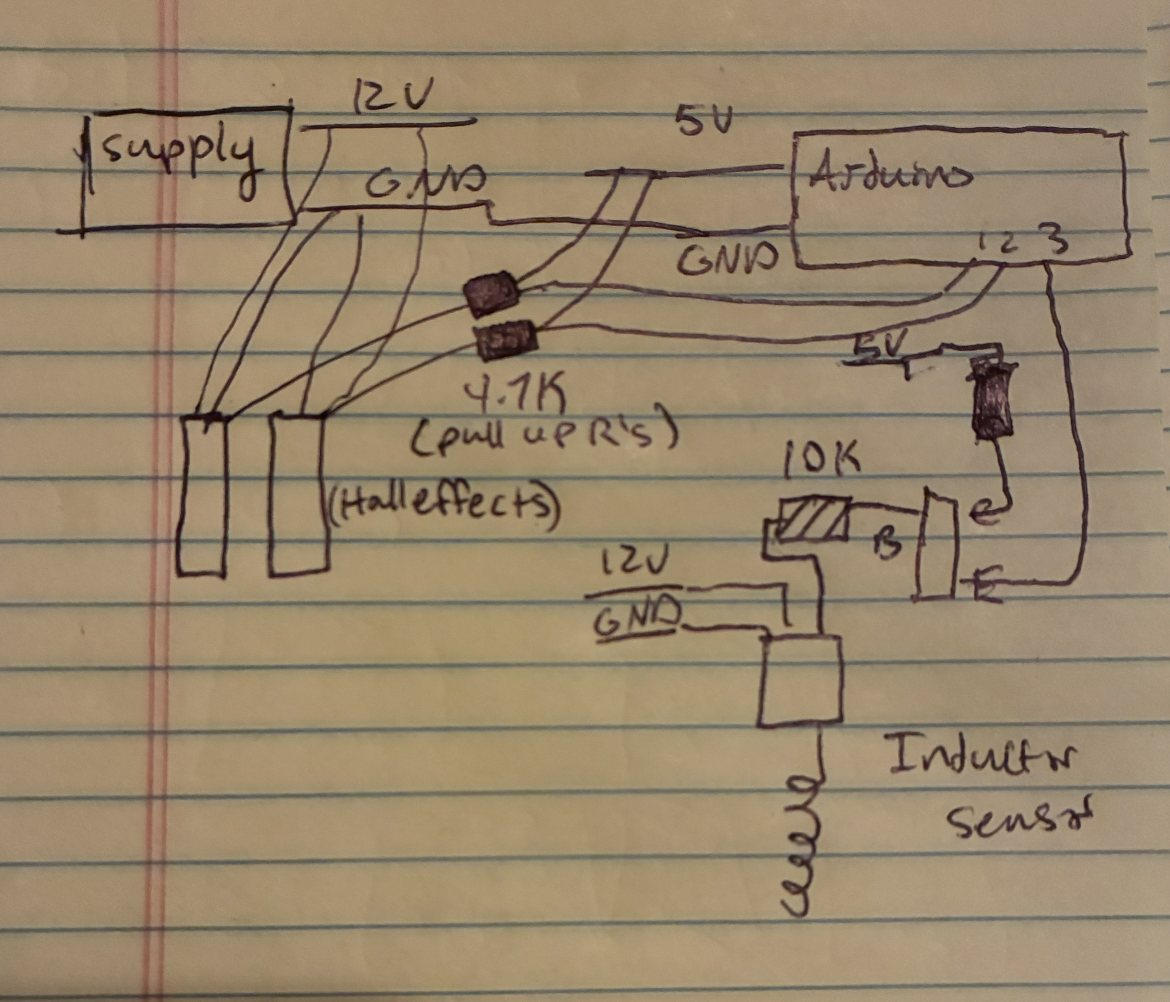
\includegraphics[height=0.40\textheight]{dyno-bench-wiring.jpg}\\[1pt]
  {\tiny\color{dim} 4.7\,k pull-ups to 5\,V; 10\,k into the base}\\[5pt]
  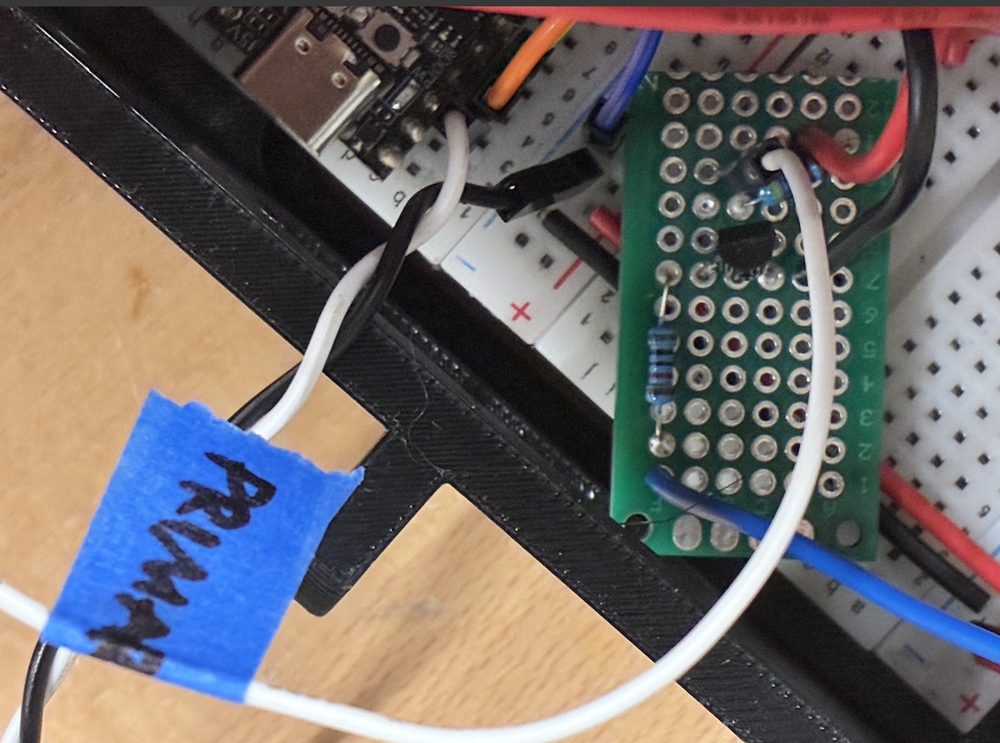
\includegraphics[height=0.29\textheight]{dyno-npn-rebuild.jpg}\\[1pt]
  {\tiny\color{dim} Rebuilt front end on perfboard}
\end{column}
\end{columns}
\end{frame}

%==============================================================================
\begin{frame}{Rear CAN node --- role and MCU selection}
\scriptsize
\begin{columns}[T,onlytextwidth]
\begin{column}{0.50\textwidth}
\textbf{What this node does}
\begin{itemize}
  \item Acquires \hd{engine RPM}, \hd{CVT secondary RPM}, \hd{two rear shock pots};
        publishes to the vehicle CAN bus. One of three nodes around the central DAQ.
\end{itemize}
\smallskip
\textbf{Why STM32G431RBTx}
\begin{itemize}
  \item \hd{Native FDCAN} --- removes an external MCP2515 and its solder joints.
        Fewer failure points on a chassis that vibrates.
  \item \hd{Hardware timer capture} (TIM2/TIM3) timestamps edges in silicon,
        removing the ISR jitter the ESP32 approach carries.
  \item \hd{FMAC accelerator} offloads shock-pot filtering, leaving CPU headroom
        for the CAN task.
  \item \hd{Ecosystem} --- same G4 family as the central node. One toolchain, one
        HAL, one debugger across every node.
\end{itemize}
\smallskip
\textbf{Rejected:} {\color{dim}ESP32-C3 (no CAN FD), ATmega328P (needs external
controller), STM32F103 ``Bluepill'' (no FDCAN + clone silicon risk).}
\end{column}
\begin{column}{0.48\textwidth}
  \centering
  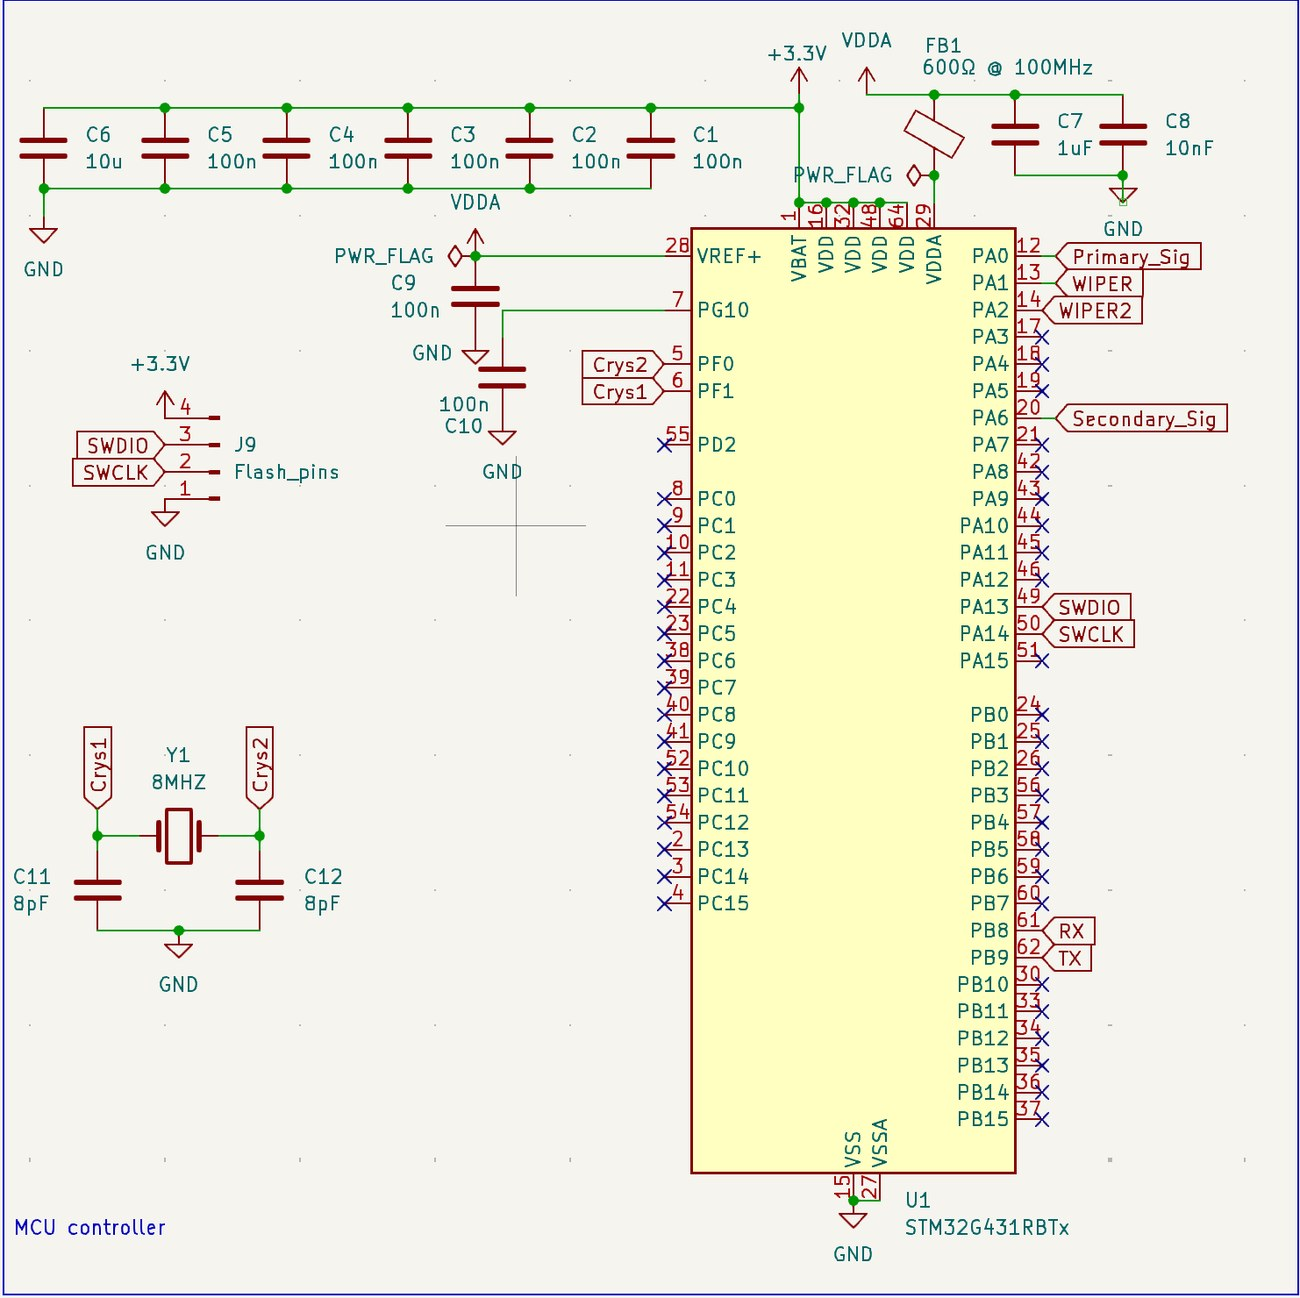
\includegraphics[height=0.72\textheight]{rn-mcu.jpg}\\[1pt]
  {\tiny\color{dim} MCU block: 100\,nF per supply pin, 10\,\textmu F bulk, 8\,MHz
   crystal, SWD header, ferrite-isolated VDDA}
\end{column}
\end{columns}
\end{frame}

%==============================================================================
\begin{frame}{Rear CAN node --- sensor front ends and analog integrity}
\scriptsize
\begin{columns}[T,onlytextwidth]
\begin{column}{0.50\textwidth}
\textbf{Both open-collector --- different voltage domains}
\begin{itemize}
  \item \hd{Primary (spark pickup, 12\,V):} open-collector, one pulse per ignition
        event, referenced to \hd{12\,V} --- $\sim$4$\times$ the MCU maximum.
        100\,k/47\,k divider, Schottky clamping to the rails, \hd{9.3\,V TVS}.
  \item \hd{Secondary (Hall, 5\,V):} same output topology, easier domain. One
        \hd{4.7\,k$\Omega$ pull-up to 3.3\,V} is the whole conditioning ---
        the pull-up's rail sets the logic-high level, so no translation stage.
        \hd{18.3\,V TVS} to ground.
\end{itemize}
\smallskip
\textbf{Shock potentiometers stay analog}
\begin{itemize}
  \item Ratiometric divider driven by the supply $\Rightarrow$ the reading
        \emph{tracks the rail}. Analog-rail cleanliness \emph{is} measurement accuracy.
\end{itemize}
\smallskip
\textbf{Analog supply integrity}
\begin{itemize}
  \item \hd{600\,$\Omega$@100\,MHz ferrite} isolating VDDA --- chosen over an
        inductor, which would resonate with the decoupling network.
  \item \hd{1\,\textmu F $\parallel$ 10\,nF} behind it: bulk plus low-ESL.
  \item 100\,nF per supply pin; VREF+ gets its own --- reference noise lands on
        every conversion.
\end{itemize}
\end{column}
\begin{column}{0.48\textwidth}
  \centering
  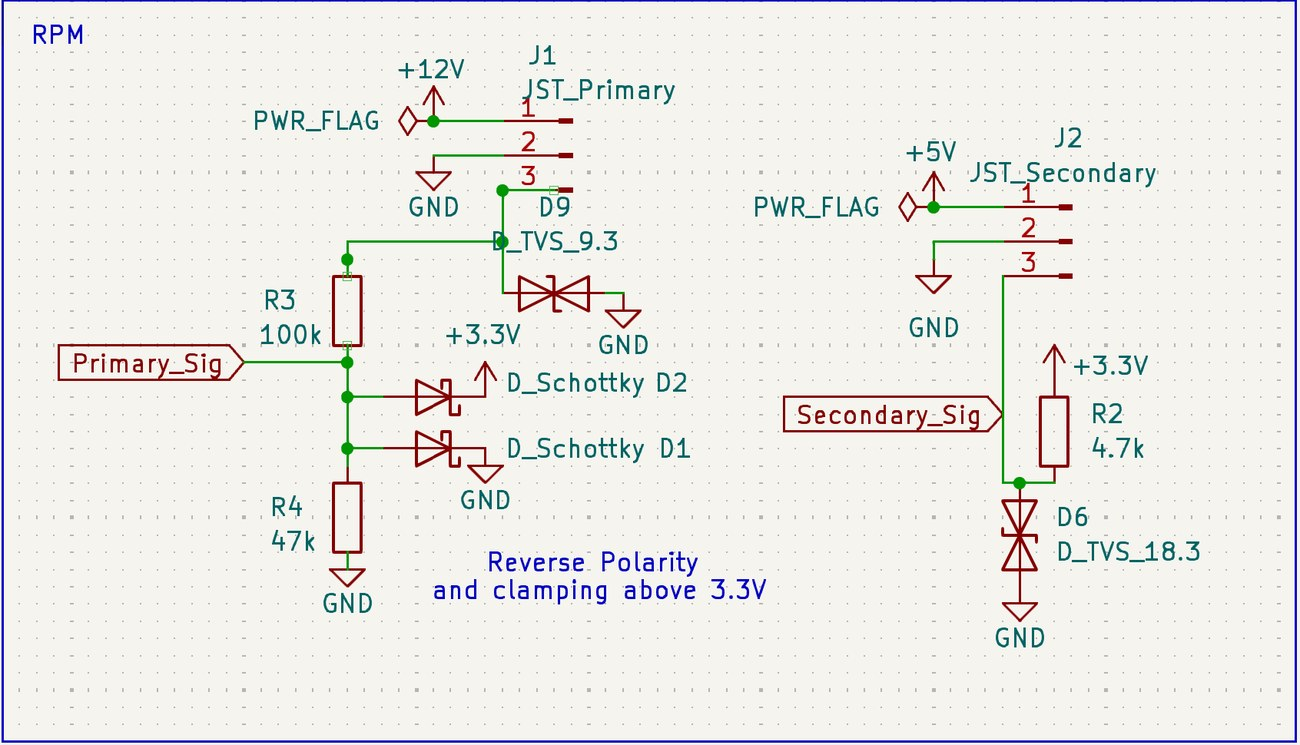
\includegraphics[height=0.38\textheight]{rn-rpm-frontends.jpg}\\[1pt]
  {\tiny\color{dim} Primary vs.\ secondary RPM conditioning}\\[5pt]
  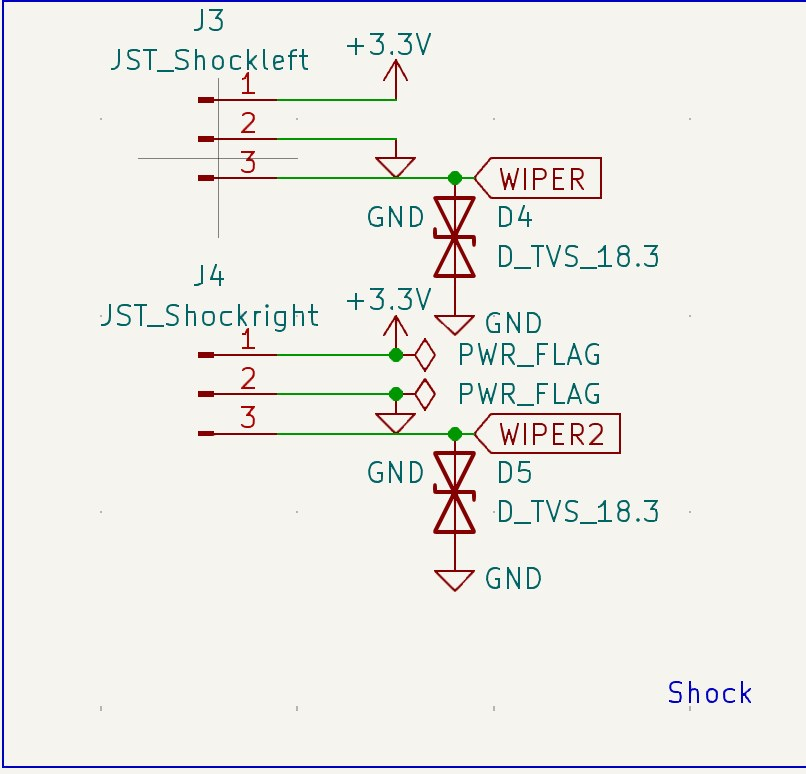
\includegraphics[height=0.26\textheight]{rn-shockpots.jpg}\\[1pt]
  {\tiny\color{dim} Shock potentiometer inputs}
\end{column}
\end{columns}
\end{frame}

%==============================================================================
\begin{frame}{Rear CAN node --- protection, layout, open items}
\scriptsize
\begin{columns}[T,onlytextwidth]
\begin{column}{0.50\textwidth}
\textbf{Every external pin is a way in}
\begin{itemize}
  \item TVS across \hd{all power rails}, \hd{both RPM inputs}, the \hd{CAN pair}
        --- every wire out is an antenna running past an ignition system.
  \item \hd{Jumper-selectable 120\,$\Omega$ termination} --- which node sits at a
        physical bus end changes with how the car is wired.
  \item \hd{LED per rail.} Turns ``the node is dead'' into ``the 5\,V rail is
        dead'' without a multimeter in the paddock.
\end{itemize}
\smallskip
\textbf{Layout:} {\color{dim}decoupling \textbf{placement} is the requirement, not the
schematic. Deutsch DT is wire-to-wire only $\Rightarrow$ Molex Micro-Fit 3.0 with
pegs on the board, DT on the harness.}\smallskip\par
\smallskip
\textbf{\color{bad}Open items --- need a decision}
\begin{itemize}
  \item \bd{Transceiver:} board shows SN65HVD230, ordering sheet has TJA1051T/3.
  \item \bd{Inductive channel:} board keeps the \emph{divider}; bench uses the
        \emph{transistor}. Re-test first.
  \item Schematic through ERC, layout routed, \hd{not fabricated}.
\end{itemize}
\end{column}
\begin{column}{0.48\textwidth}
  \centering
  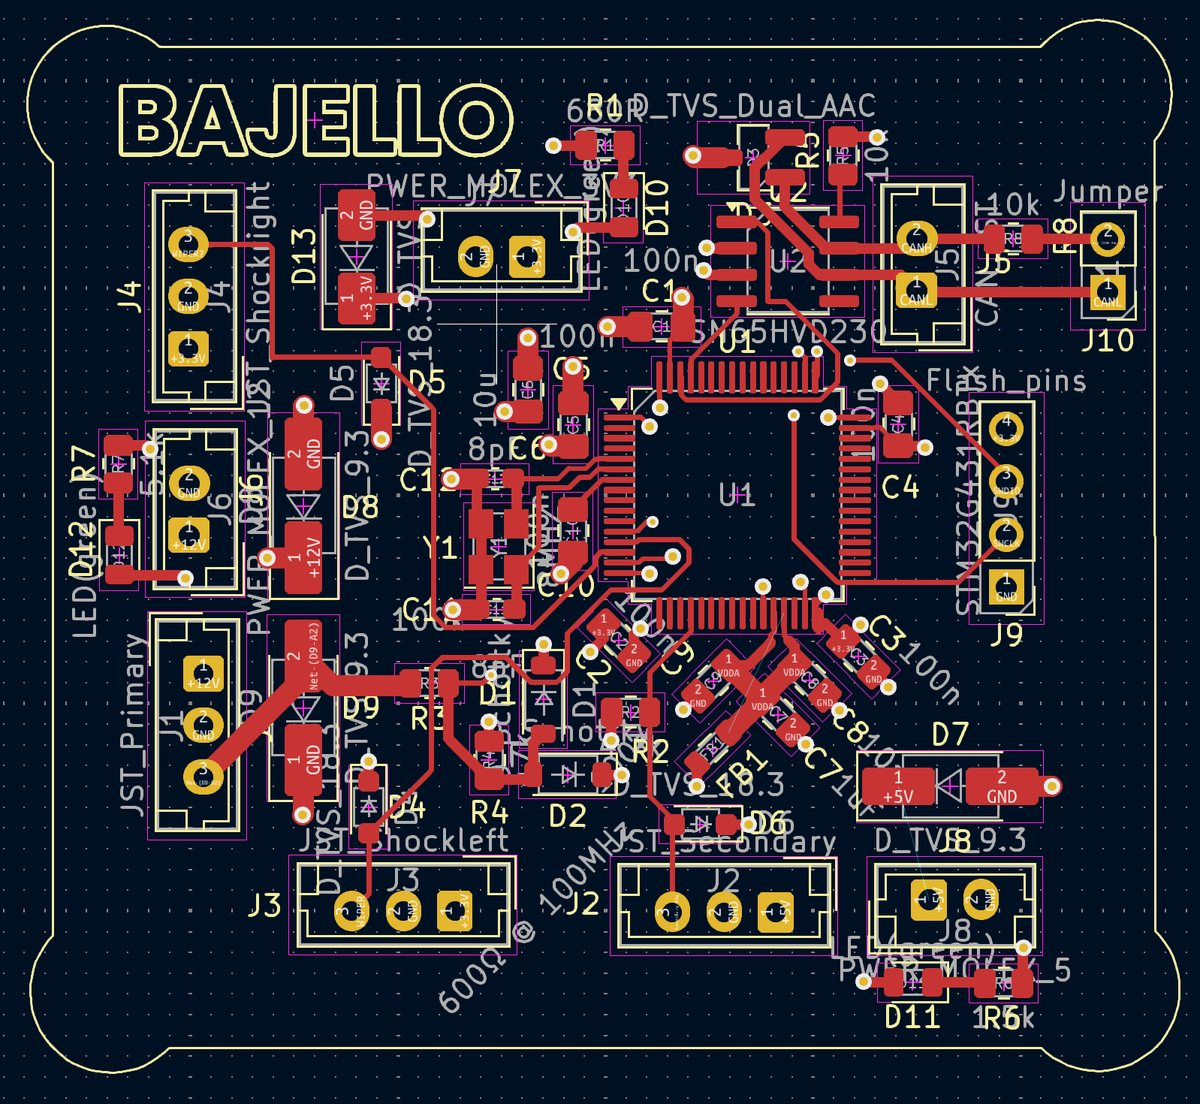
\includegraphics[height=0.70\textheight]{rn-layout-signal.jpg}\\[1pt]
  {\tiny\color{dim} Layout with power and ground planes hidden --- the view that
   shows whether signal routing is sane}
\end{column}
\end{columns}
\end{frame}

%==============================================================================
% SPEAKER SCRIPTS
%==============================================================================
{\setbeamertemplate{footline}{}
\begin{frame}{Speaker script --- Slide 1: inductive front end}
\scriptsize
\textit{\color{dim}$\sim$60 seconds. Lead with the failure. This is the slide reviewers
will ask about.}
\medskip

``This is the part of the design I got wrong the first time, so I want to walk
through it directly.

The inductive pickup clamps onto the ignition lead and gives one open-collector
pulse per spark, referenced to its 12-volt supply --- roughly four times the
microcontroller's absolute maximum. I read that as a level problem and reached for a
divider: 147 kilohms total, drawing only 82 microamps, on the assumption that a light
load would leave the signal intact.

On the bench the logic-high sagged to 2.4 volts, below threshold.

The mistake wasn't the resistor values --- it was the topology. An open-collector
output has no internal path to pull its line \emph{high}; it only sinks. A divider
attenuates a signal that is actively being driven, and this one never was. Different
resistor values would not have fixed it.

The right circuit uses the sensor as a switch and translates domains. A 2N3904: the
sensor's 12-volt open-collector output drives the base through 10 kilohms on about
0.38 milliamps, and the transistor pulls a 3.3-volt-pulled-up MCU pin low. The
12-volt domain never touches the microcontroller.

One thing to flag: the transistor inverts, so timer capture has to trigger on the
rising edge --- the sensor \emph{releasing}, not firing. Easy to get backwards in
firmware.

The general lesson: read the output \emph{topology} before choosing a conditioning
circuit. Open-collector, push-pull and passive outputs each fail differently, and a
divider is only correct for one of them.''
\end{frame}

\begin{frame}{Speaker script --- Slide 2: role and MCU selection}
\scriptsize
\textit{\color{dim}$\sim$50 seconds. This is the ``why this part'' slide --- reviewers
want the reasoning, not the datasheet.}
\medskip

``The rear node acquires engine RPM, CVT secondary RPM, and the two rear shock
potentiometers, then publishes them onto the vehicle bus. It's one of three nodes
around the central DAQ.

I selected the STM32G431RBTx against our weighted decision matrix, and there were
four reasons.

Native FDCAN was the big one. It removes an external MCP2515 and every solder joint
that comes with it, and on a chassis that vibrates the joint count is a real
reliability term.

Second, hardware timer capture. TIM2 and TIM3 timestamp sensor edges in silicon, so
we don't carry the interrupt-latency jitter that the software approach on the dyno
ESP32 has.

Third, the FMAC filter accelerator offloads shock-pot conditioning from the CPU,
which leaves headroom for the CAN task.

Fourth --- and this one is about the team, not the chip --- the central node is the
same G4 family. One toolchain, one HAL, one debugger across every node, so anyone
who can work on one node can work on all of them.

On what I rejected: the ESP32-C3 has no CAN FD and would fragment the toolchain.
The ATmega328P needs an external CAN controller. And the STM32F103 Bluepill has no
FDCAN, plus the widely-sold clones carry counterfeit-silicon risk that our
35-percent durability weighting can't accept.''
\end{frame}

\begin{frame}{Speaker script --- Slide 3: front ends and analog integrity}
\scriptsize
\textit{\color{dim}$\sim$60 seconds. The point to land: signal type, not sensor name,
determines the circuit.}
\medskip

``Both RPM channels are open-collector --- both sink current, neither sources it.
What separates them is the voltage domain they're referenced to, and that's what
decides the circuit.

The primary is the spark pickup. It clamps the ignition lead and gives one
open-collector pulse per ignition event, but it's referenced to its 12-volt supply
--- about four times the MCU's absolute maximum. So it can't touch the pin directly
no matter how clean the pulse is. On this board that's a 100k/47k divider, Schottky
diodes clamping to the rails, and a 9.3-volt TVS at the connector.

The secondary is the Hall sensor: same output topology, much easier domain. It runs
on 5 volts and one 4.7k pull-up is the entire signal conditioning. The detail worth
noting is that the pull-up's rail --- not the sensor's supply --- sets the logic-high
level the MCU sees, so pulling it to 3.3 volts means no translation stage at all.
Plus an 18.3-volt TVS.

The shock pots are the third case: they stay analog all the way to the ADC. A
potentiometer is a ratiometric divider, so its reading tracks the supply rail
directly --- which means the cleanliness of the analog rail \emph{is} the accuracy of
the measurement.

That's why the analog supply gets its own treatment. A 600-ohm-at-100-megahertz
ferrite isolates VDDA. I chose a ferrite over an inductor specifically because an
inductor would form a resonant tank with the decoupling caps and ring. Behind it,
1 microfarad in parallel with 10 nanofarads --- the big one for bulk load steps, the
small one because it has lower ESL and still works where the big one has gone
inductive. Then 100 nanofarads per supply pin, and VREF+ gets its own, because noise
on the ADC reference shows up on every single conversion.''
\end{frame}

\begin{frame}{Speaker script --- Slide 4: protection, layout, open items}
\scriptsize
\textit{\color{dim}$\sim$60 seconds. End on the open items --- that is what you want the
room to respond to.}
\medskip

``The theme on protection is that every wire leaving this board is a long antenna
running past an ignition system, and every connector is a path for a transient the
MCU won't survive. So there's TVS across all power rails, both RPM inputs, and the
CAN pair.

Bus termination is on a jumper rather than a fixed resistor, because which node sits
at a physical end of the bus changes with how the car gets wired that season. And
there's an LED on every rail --- cheap, and it turns `the node is dead' into `the
5-volt rail is dead' without unpacking a multimeter in the paddock.

On layout: the image here has the power and ground planes hidden, which is the view
that actually shows whether the routing is sane --- with the pours on, everything
looks connected. The decoupling requirement is placement, not schematic; each cap
has to sit within a few millimetres of its pin or the bond-wire inductance it exists
to cancel just wins. And connectors are a pigtail --- Deutsch DT has no PCB-mount
variant, so the board carries Molex Micro-Fit 3.0 with mounting pegs and the DT
lives on the harness, with the pegs putting vibration load into the board instead of
the solder joints.

Status: schematic complete through ERC, layout routed, not fabricated. I have two
open items I want input on before it is.

First, the board currently shows an SN65HVD230 transceiver, but the ordering sheet
has the TJA1051T/3 marked as ordered. Similar footprint, but the slope-control pin
on one is a mode input on the other. That needs reconciling before we commit to a
fab run.

Second, the board still uses the divider on the inductive channel while the bench
version uses the transistor. Given that the divider is the wrong topology for an
open-collector output --- there's nothing driving the line high for it to attenuate
--- I'd like that re-tested against the actual sensor before this revision goes
out.''
\end{frame}
}

\end{document}
